\documentclass{article}
\usepackage[utf8]{inputenc}
\usepackage[letter, margin=1in]{geometry}
\usepackage{hyperref}
\hypersetup{colorlinks,urlbordercolor=blue,urlcolor=blue,pdfborderstyle={/S/U/W 1}}
\usepackage[colorinlistoftodos]{todonotes}
\title{Middelpos/SAMTEX Notes}
\author{Bob Weigel and Pierre Cilliers}
\date{June 2020}

\usepackage{natbib}
\usepackage{graphicx}

\begin{document}

\todo[inline]{Here's an inline comment.}

\section{Introduction}

%The Laboratory for Electromagnetic Innovations (LEMI) is hereby acknowledged for the use of the  magnetotelluric (MT) processing software made available to SANSA Space Science in Hermanus”.


\begin{figure}[h!]
\centering
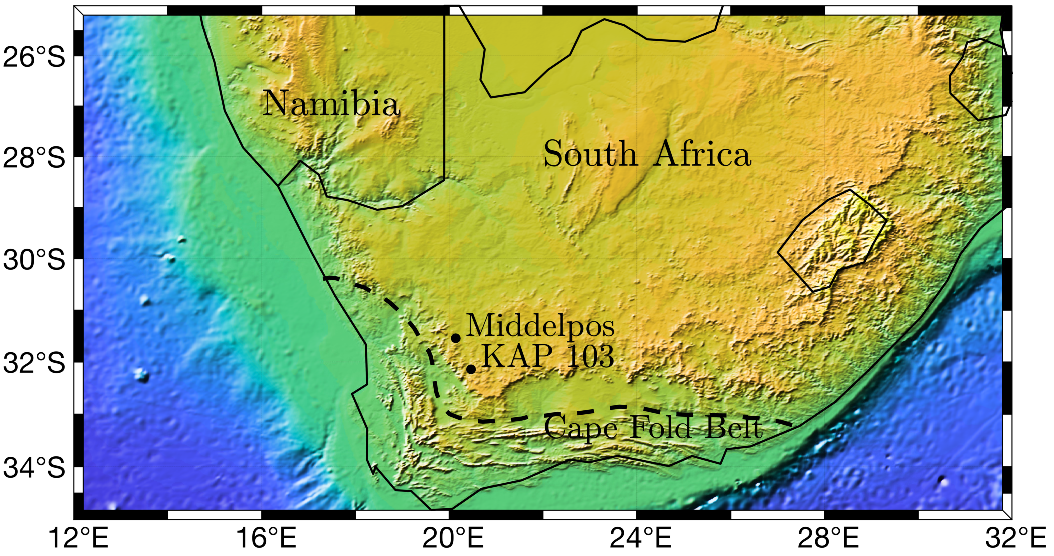
\includegraphics[width=\textwidth]{figures/map.pdf}
\caption{Location of Middelpos [$-31.544^\circ$, $20.141^\circ$] and KAP103 [$-32.139^\circ$, $20.468^\circ$] MT stations. Relief map is from \href{ngdc.noaa.gov/mgg/global/global.html}{the ETOPO1 Global Relief Model} and the Cape Fold Belt line was derived from digitization of Figure 1. of \href{https://agupubs.onlinelibrary.wiley.com/doi/pdf/10.1029/2000GL012587}{Nguuri et al., 2001}.}
\label{fig:map}
\end{figure}

\clearpage

\section{KAP103 comparison}

\begin{figure}[h!]
\centering
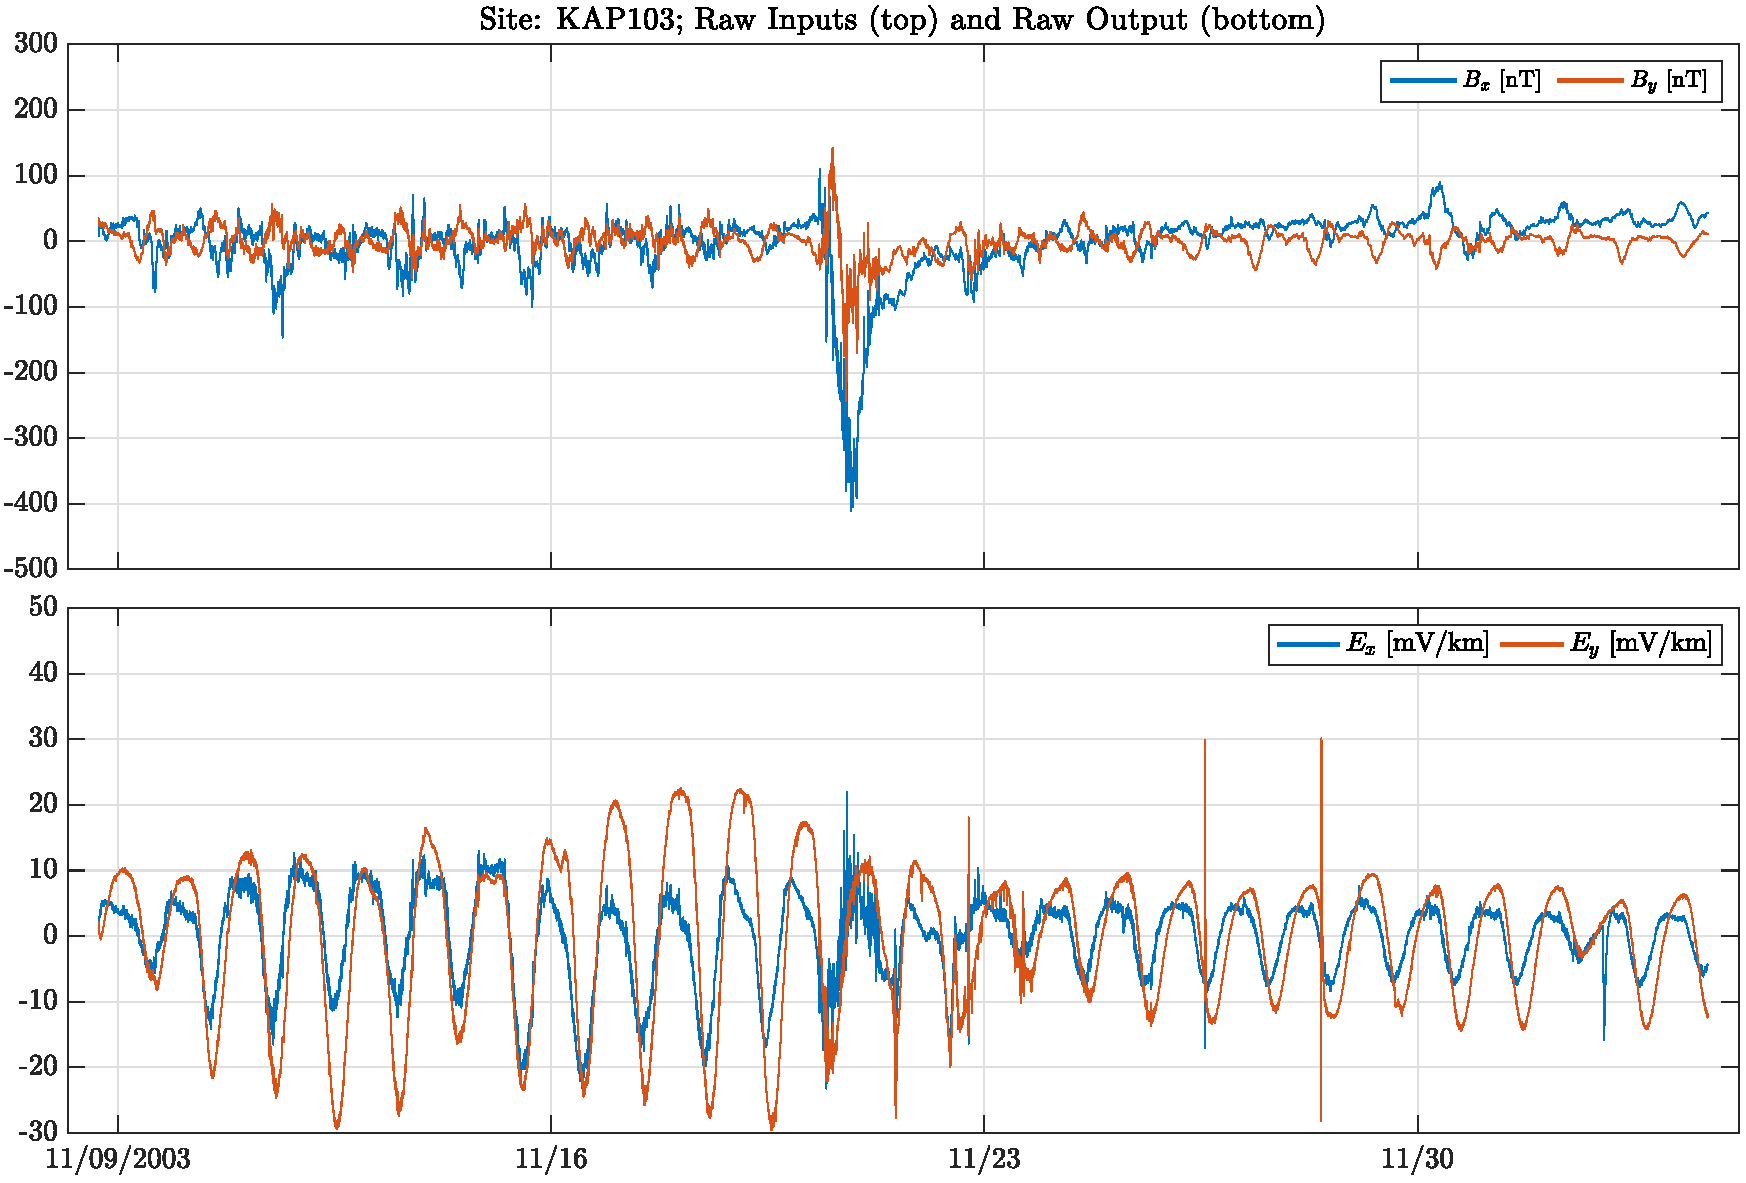
\includegraphics[width=\textwidth]{figures/KAP103/timeseries.pdf}
\caption{5-second-cadence measurements from the \href{https://www.mtnet.info/data/samtex/samtex.html}{MTNet SAMTEX page}.}
\label{fig:KAP103_timeseries}
\end{figure}

\clearpage

Legend labels

\begin{itemize}

    \item OLS 26 1-day segments - Average of 26 1-day TF estimates. Time series data used for calculation are at 5-second cadence from a LEMI-417M unit. Transfer function estimates were made using the standard OLS method in the frequency domain using logarithmically spaced evaluation frequencies (indicated by dots in the following figures).

    \item OLS One 26-day segment - TF computed using full 26-day time span of available data. Time series data and method used is the same as above.

    \item BIRRP - TF estimate derived using the Bounded Influence Remote Reference Program using sub-millisecond data (not available).

\end{itemize}

\begin{figure}[h!]
\centering
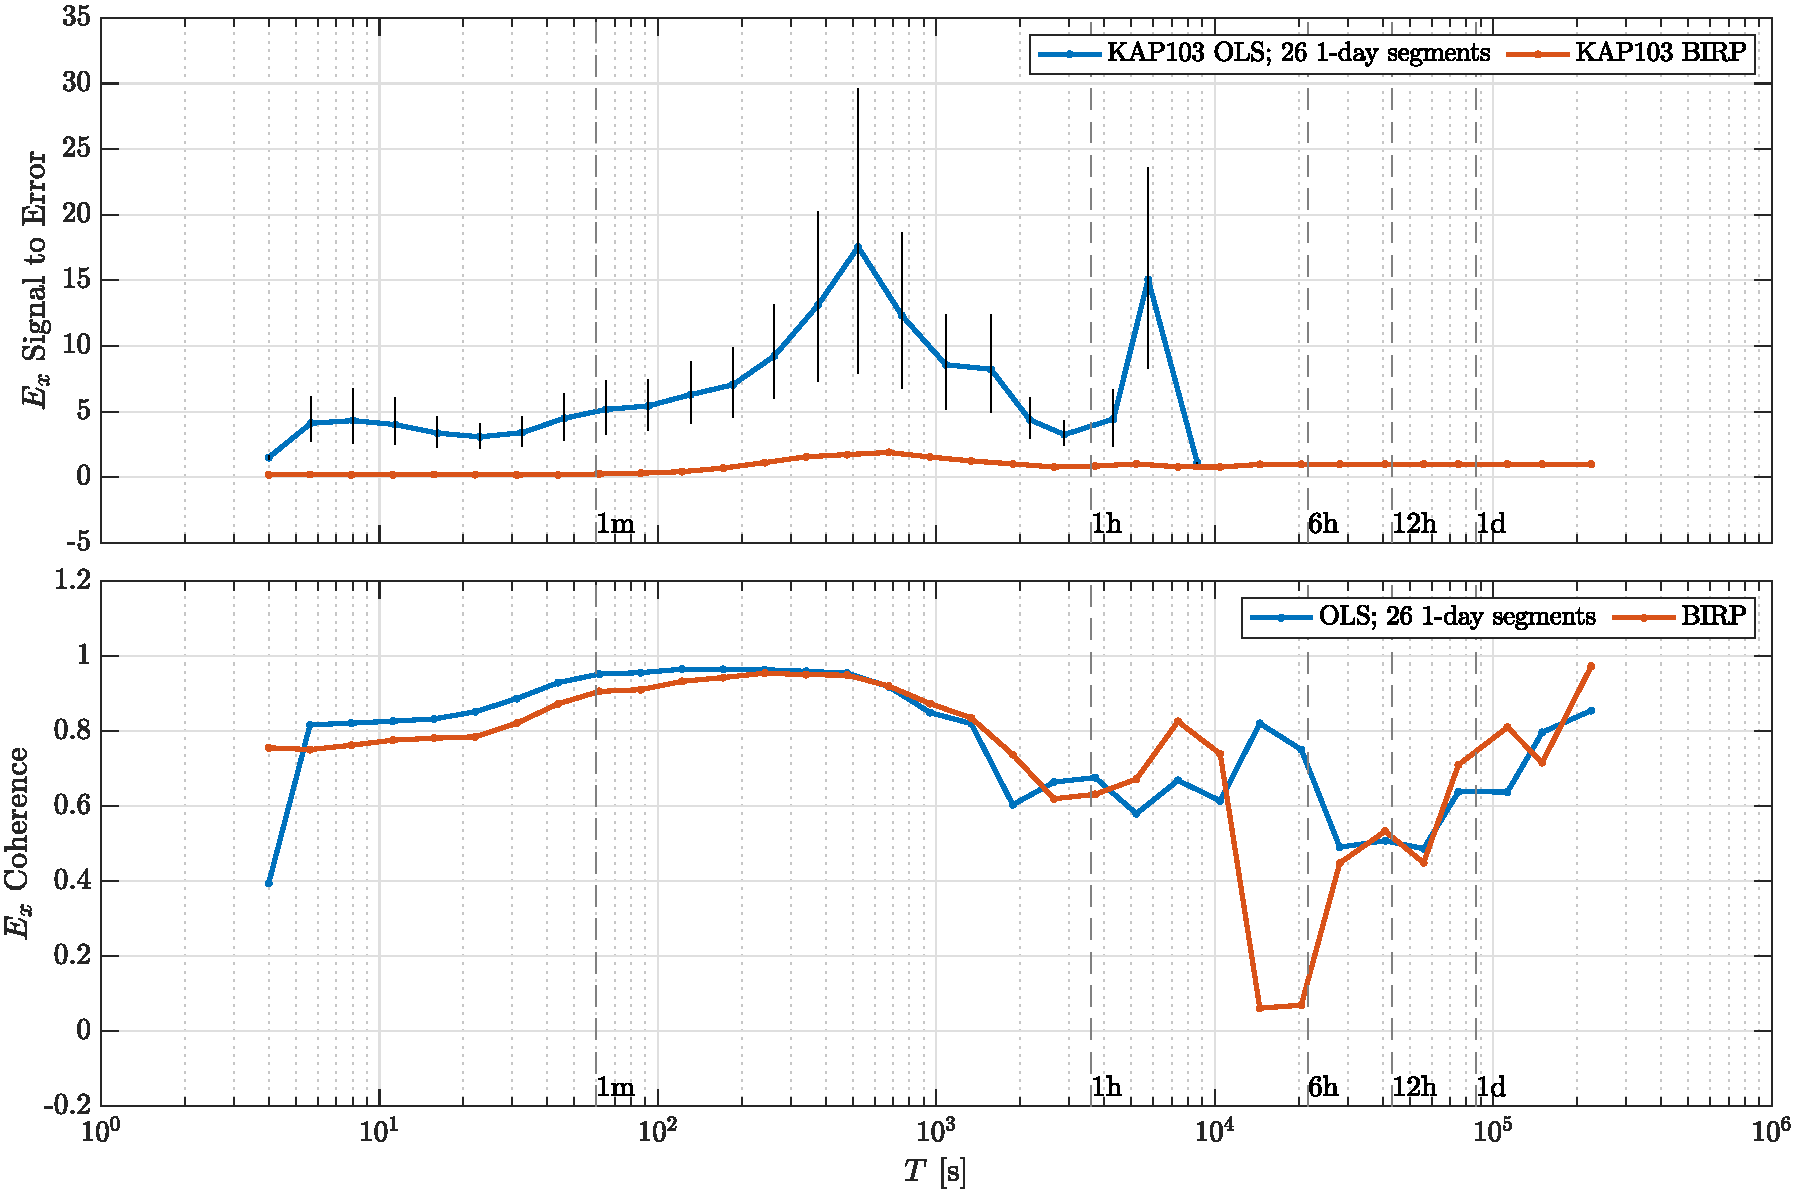
\includegraphics[width=\textwidth]{figures/KAP103/SN_compare-E_x.pdf}
\caption{(top) Signal to Error ratio versus period. The signal is the raw spectrum of the 5-second cadence measured $E_x$ averaged in bins centered on the evaluation frequencies used for the TF estimates. The error spectrum was computed by first computing the difference between the 5-second cadence predicted and measured $E_x$ and then computing its raw spectrum and averaging in bins centered on the evaluation frequencies used for the TF estimates. The ratio of these signal and error spectra are shown. (bottom) Coherence averaged in bins centered on the evaluation frequencies used for the TF estimates.}
\label{fig:universe}
\end{figure}

\begin{figure}[h!]
\centering
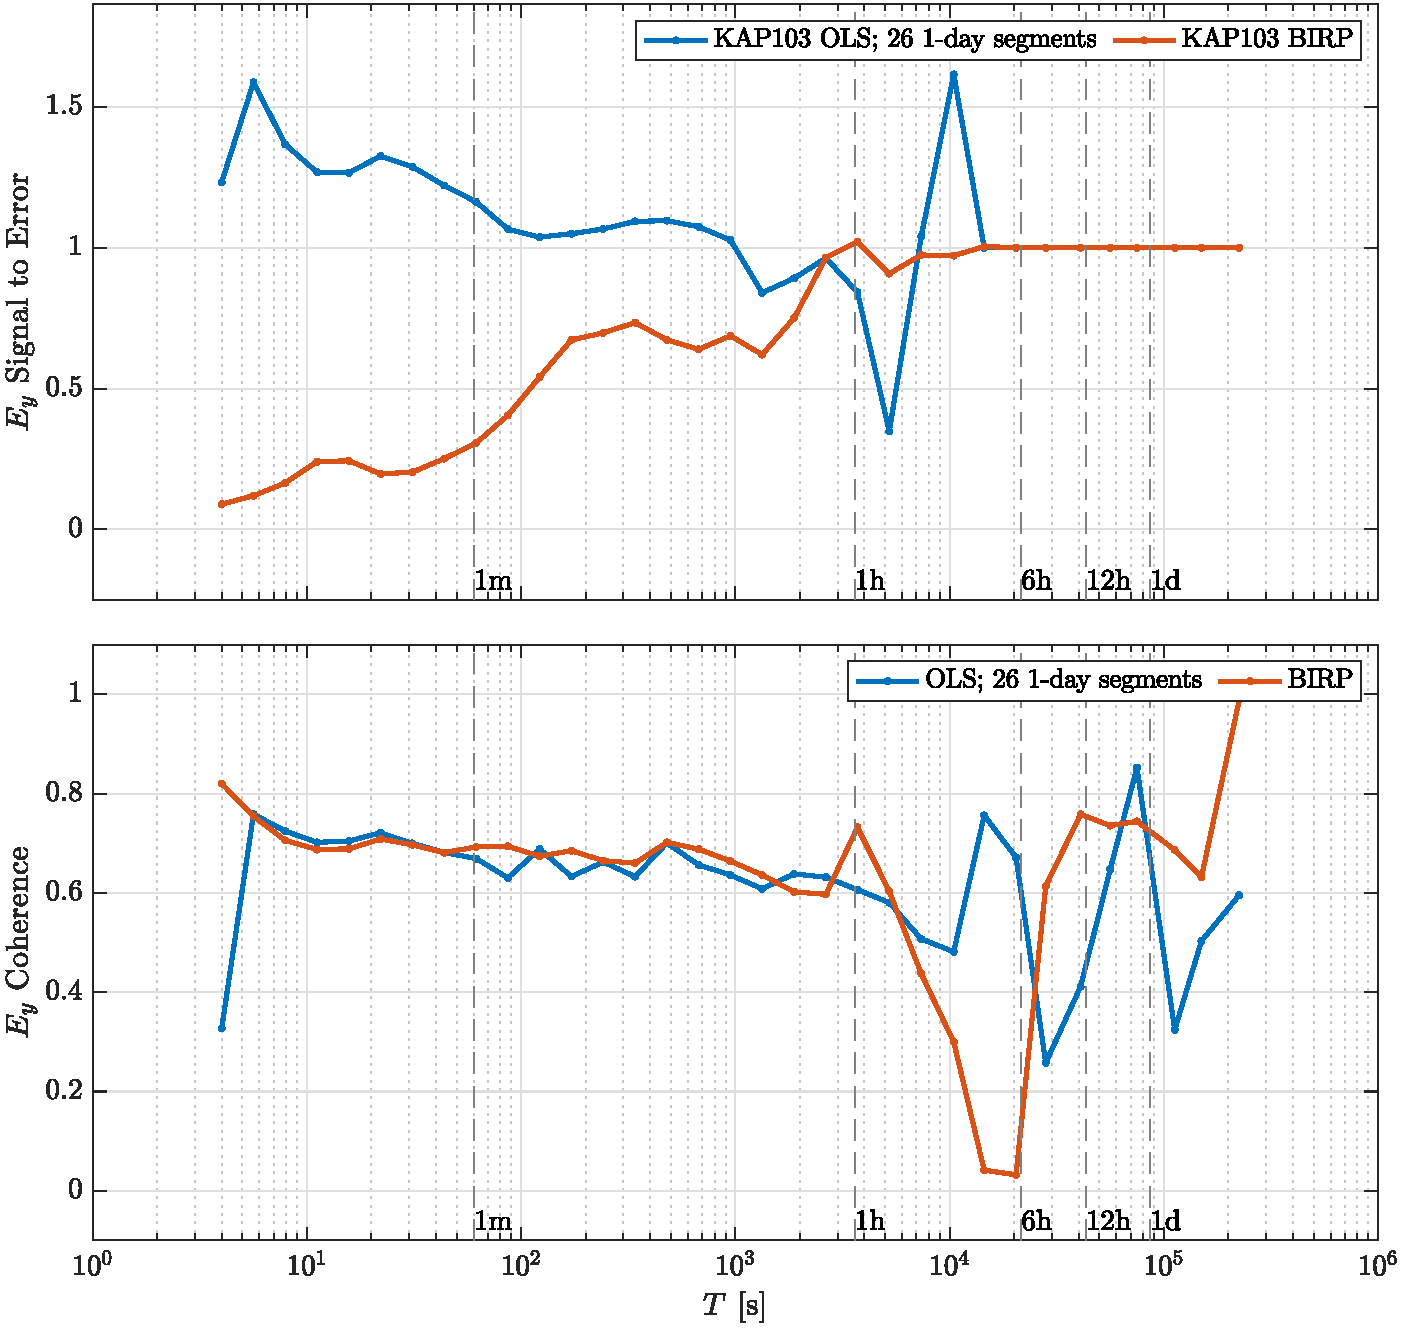
\includegraphics[width=\textwidth]{figures/KAP103/SN_compare-E_y.pdf}
\caption{Signal to Error and coherence for $E_y$.}
\label{fig:universe}
\end{figure}

\clearpage

\begin{figure}[h!]
\centering
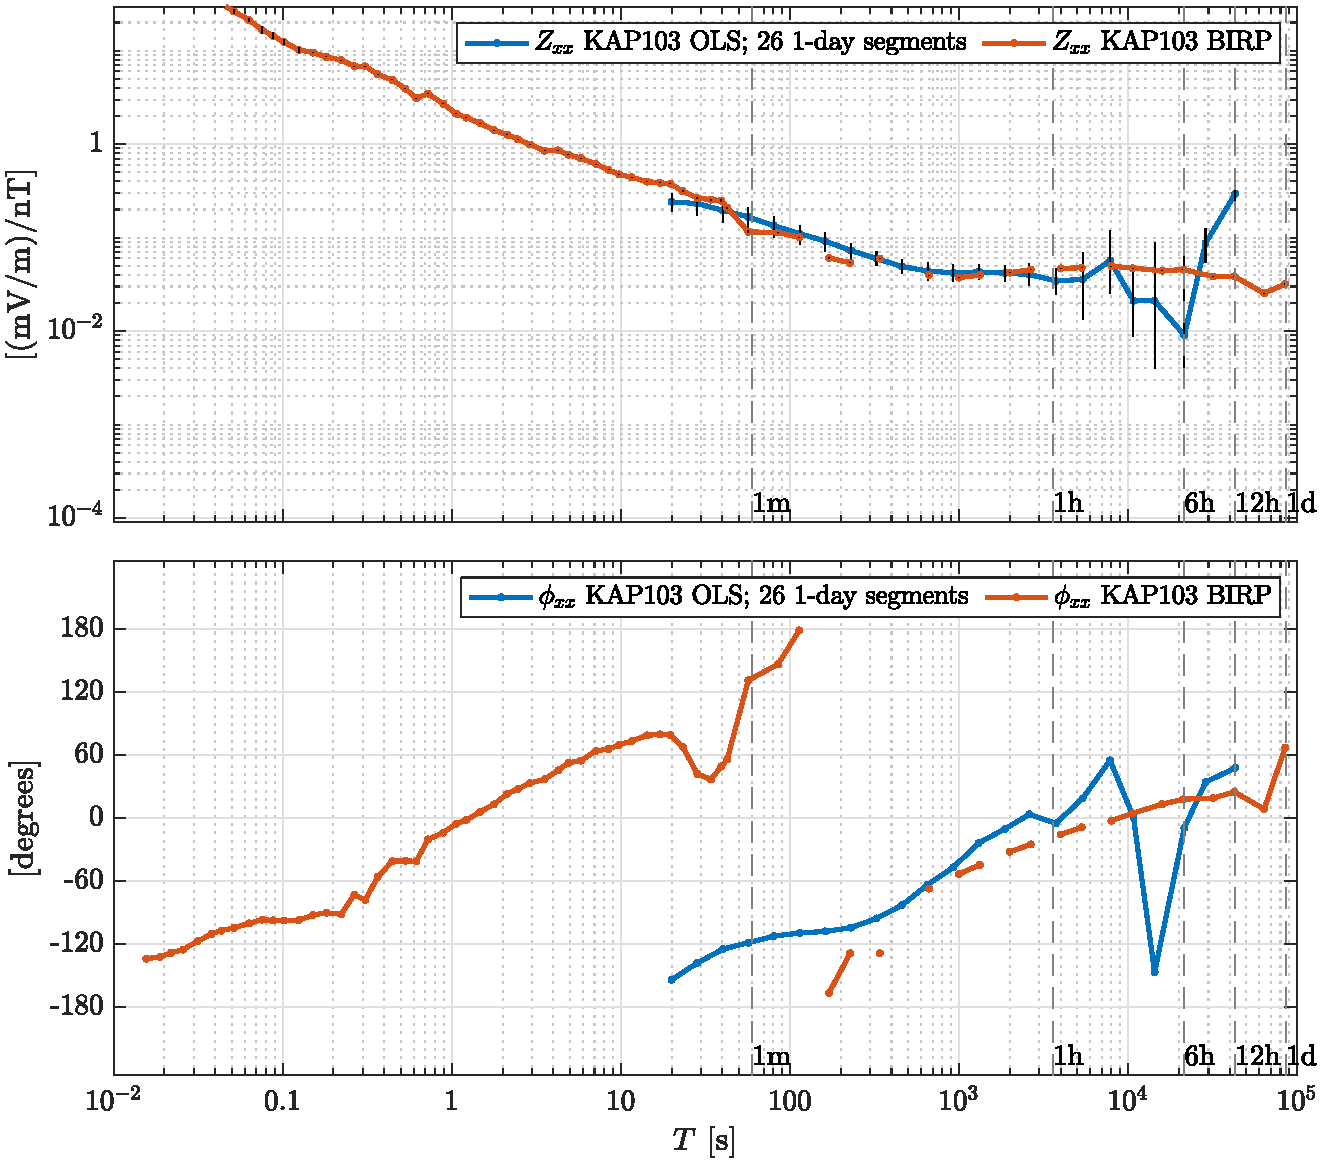
\includegraphics[width=\textwidth]{figures/KAP103/transferfnZ_compare-Z_xx_Magnitude_Phase.pdf}
\caption{}
\end{figure}


\clearpage

\begin{figure}[h!]
\centering
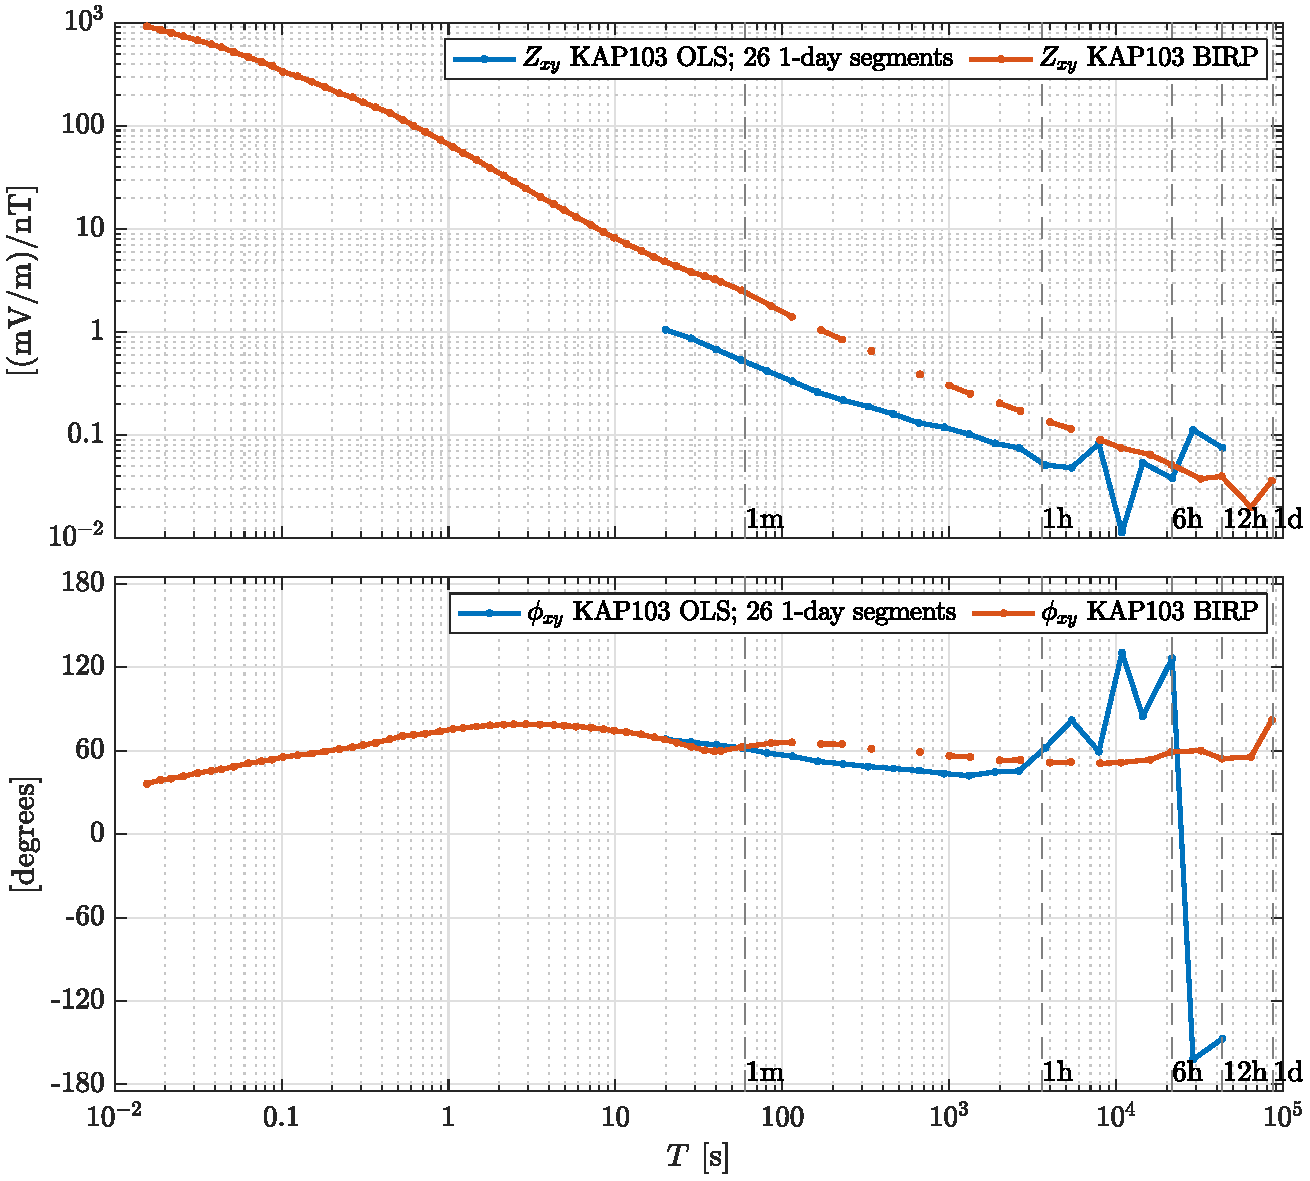
\includegraphics[width=\textwidth]{figures/KAP103/transferfnZ_compare-Z_xy_Magnitude_Phase.pdf}
\caption{}
\label{fig:universe}
\end{figure}

\begin{figure}[h!]
\centering
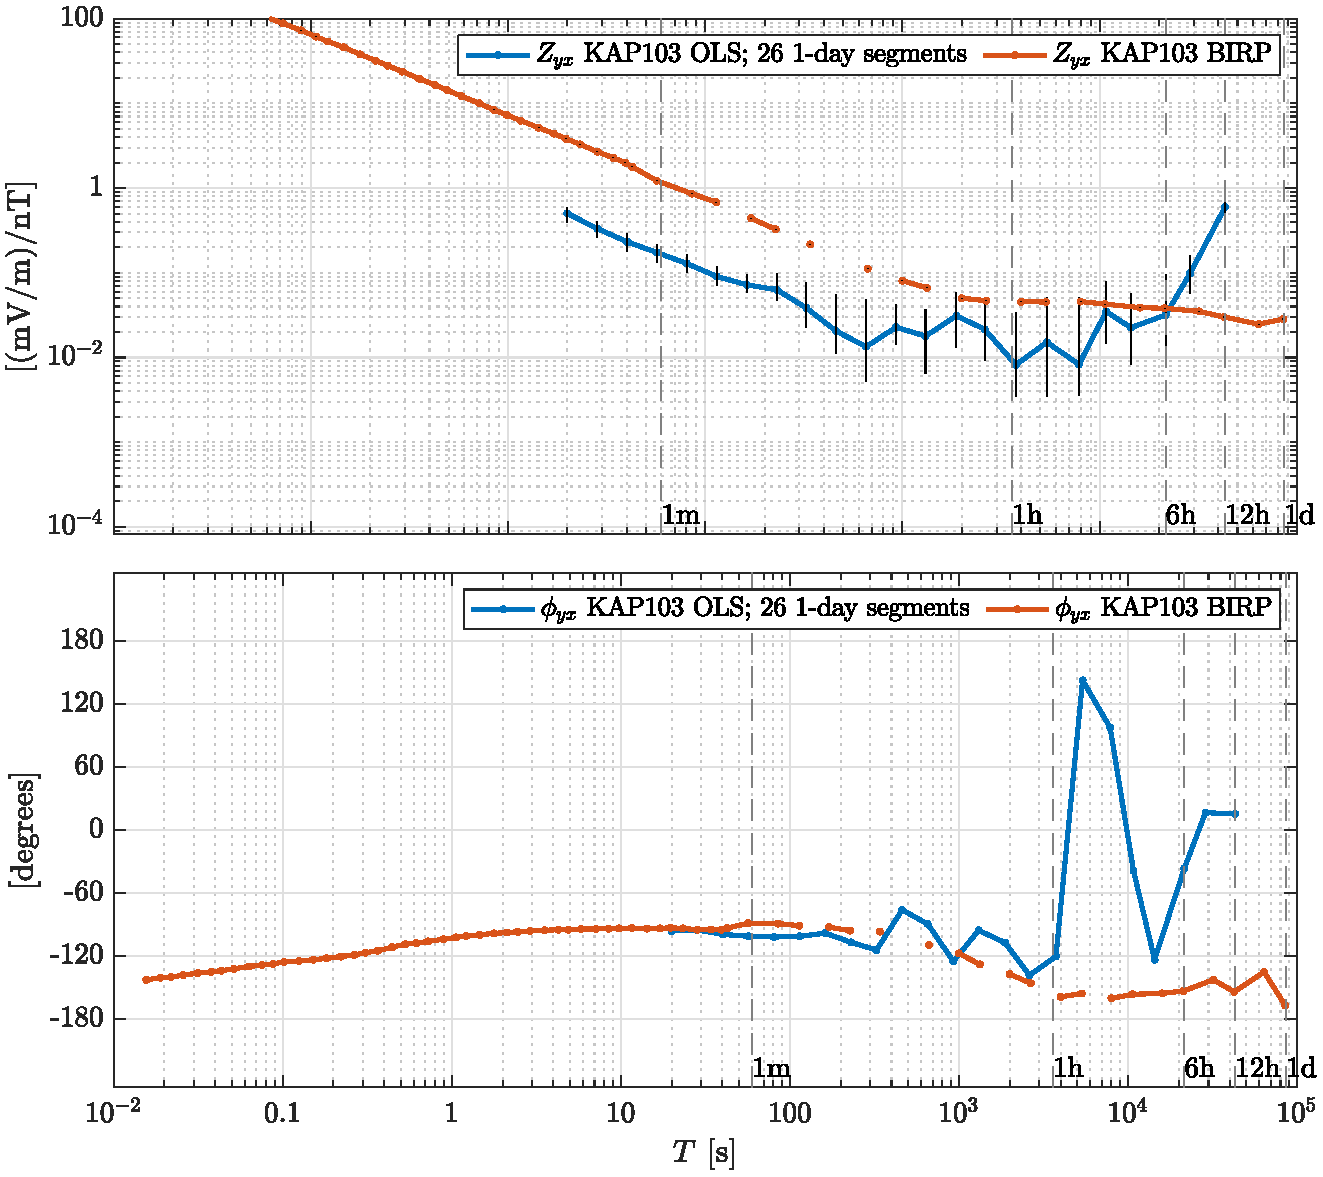
\includegraphics[width=\textwidth]{figures/KAP103/transferfnZ_compare-Z_yx_Magnitude_Phase.pdf}
\caption{}
\label{fig:universe}
\end{figure}

\begin{figure}[h!]
\centering
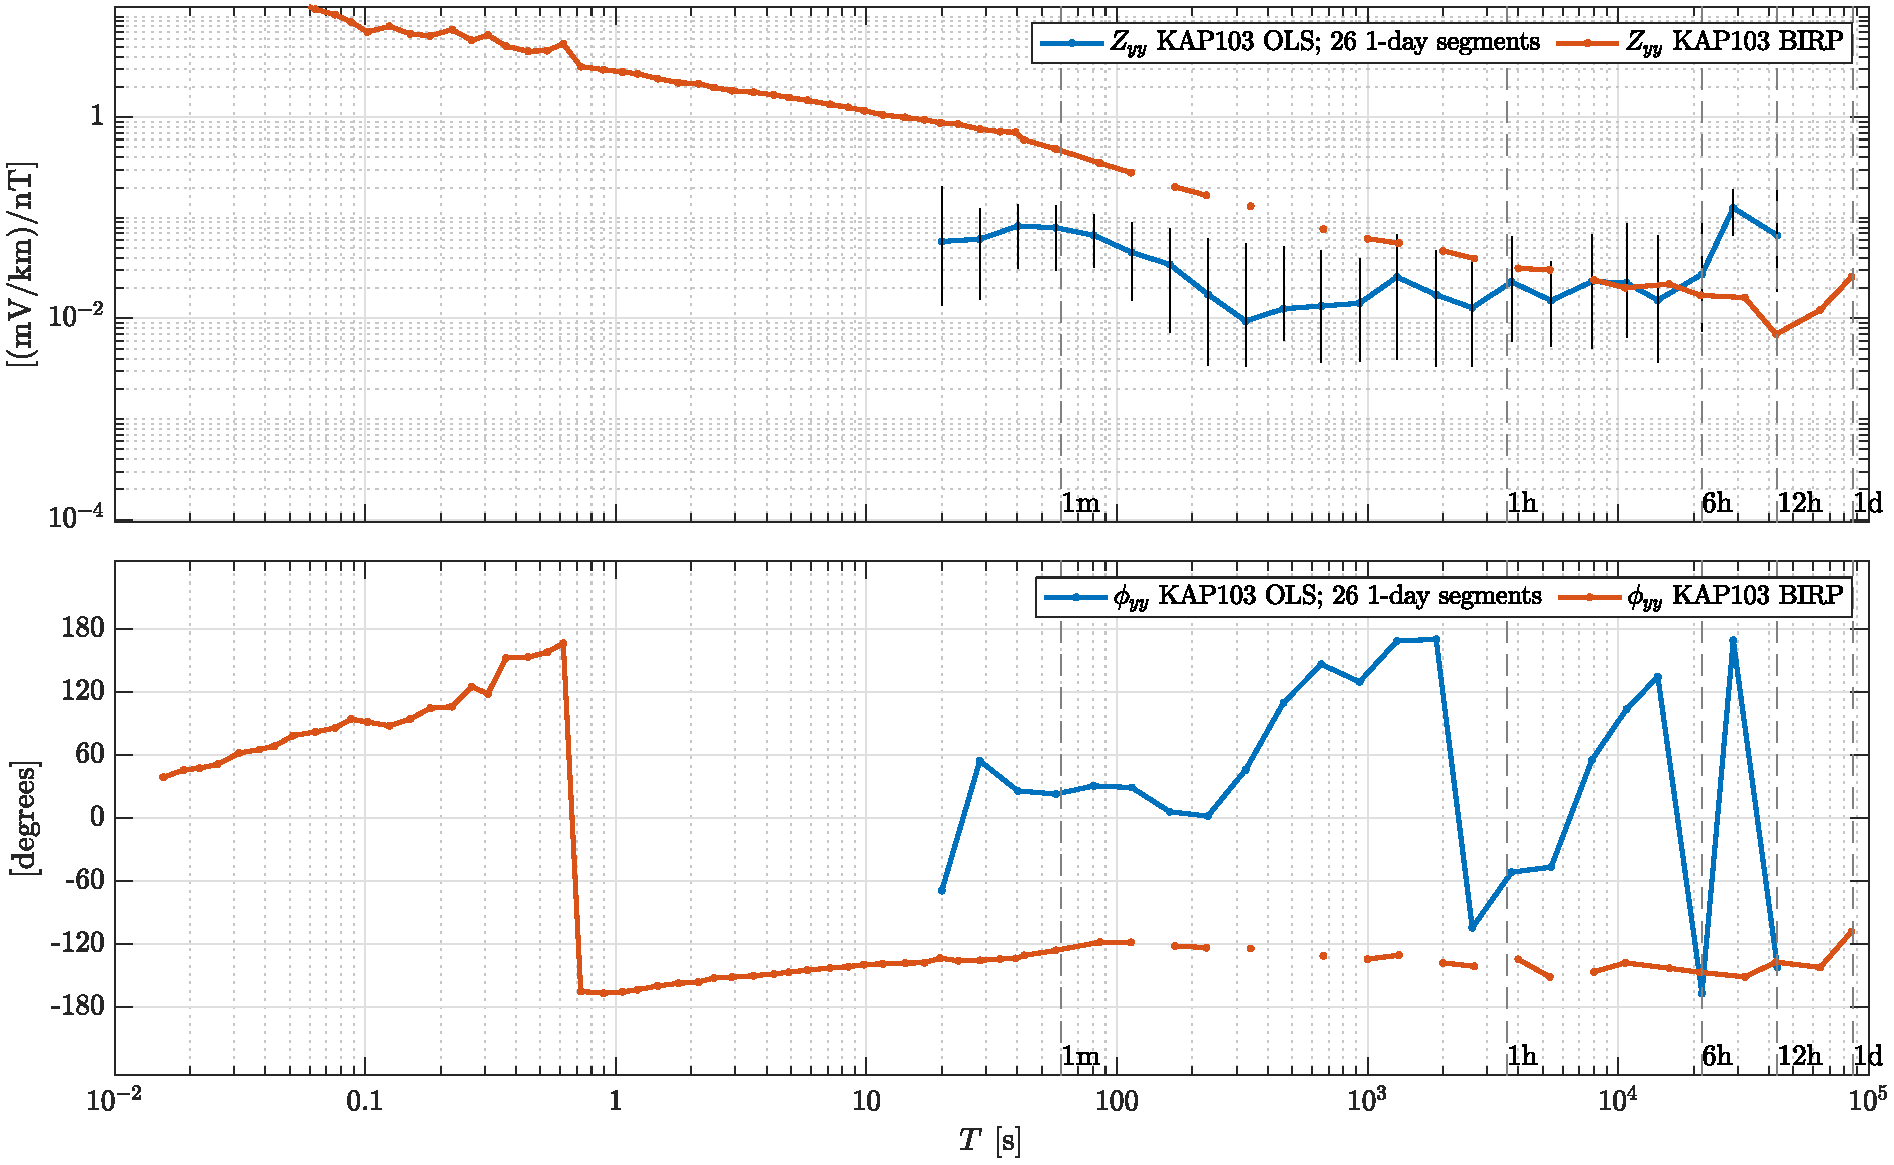
\includegraphics[width=\textwidth]{figures/KAP103/transferfnZ_compare-Z_yy_Magnitude_Phase.pdf}
\caption{}
\label{fig:universe}
\end{figure}

\clearpage

\section{Middelpos/KAP103 comparison}

\begin{figure}[h!]
\centering
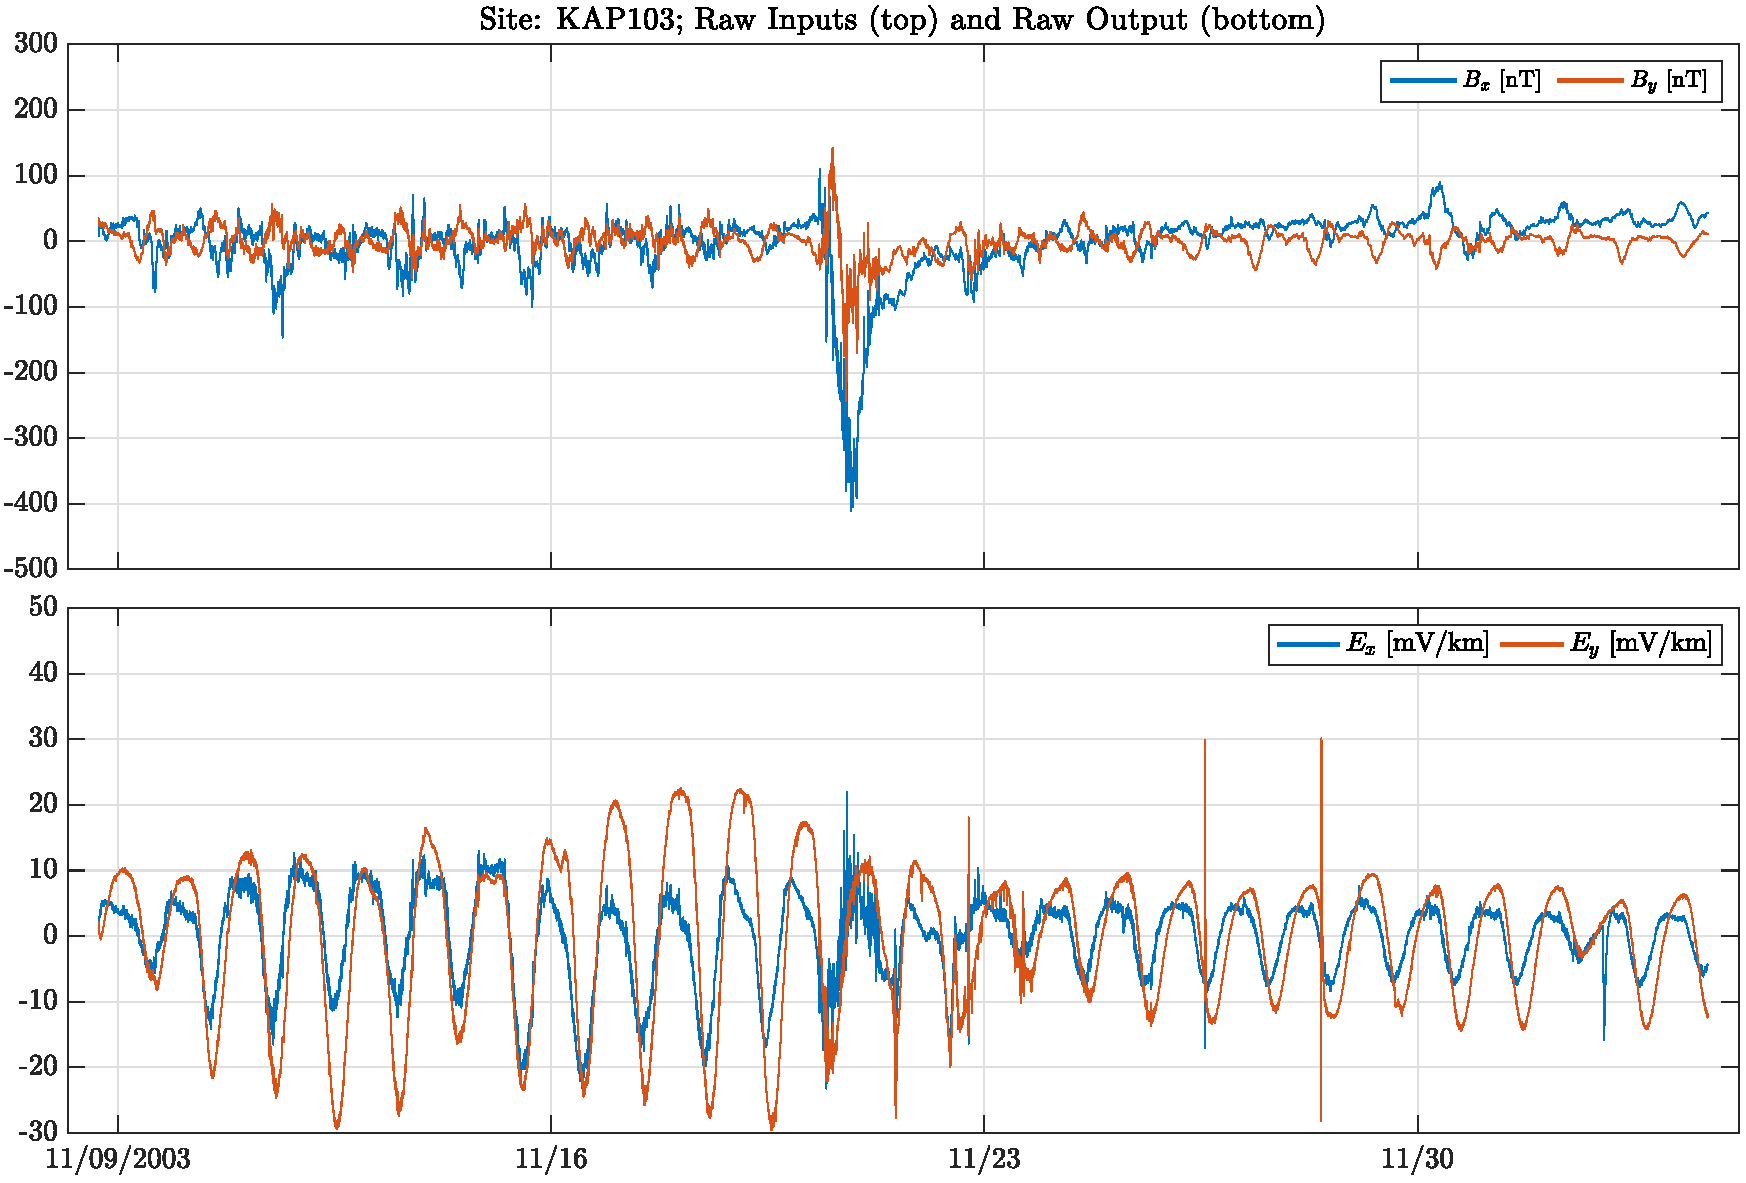
\includegraphics[width=\textwidth]{figures/KAP103/timeseries.pdf}
\caption{1-second-cadence measurements from a LEMI-417M unit in Middelpos, South Africa}
\label{fig:Middelpos_timeseries}
\end{figure}

\begin{figure}[h!]
\centering
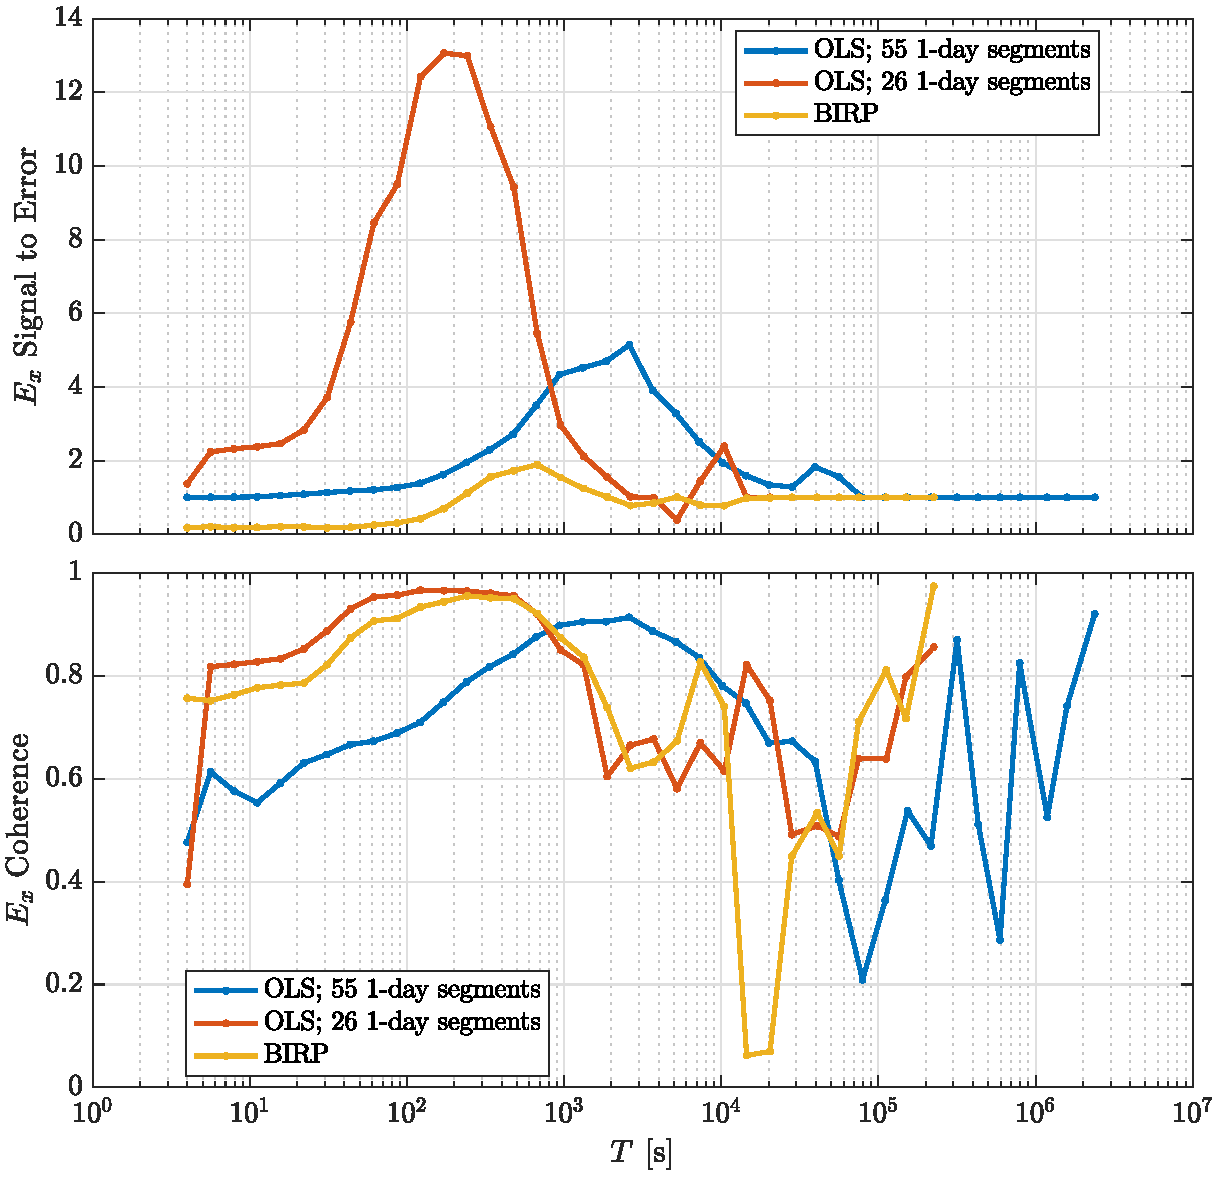
\includegraphics[width=\textwidth]{figures/KAP103_Middelpos/SN_compare-E_x.pdf}
\caption{}
\label{fig:SN_Ex_Compare}
\end{figure}

\begin{figure}[h!]
\centering
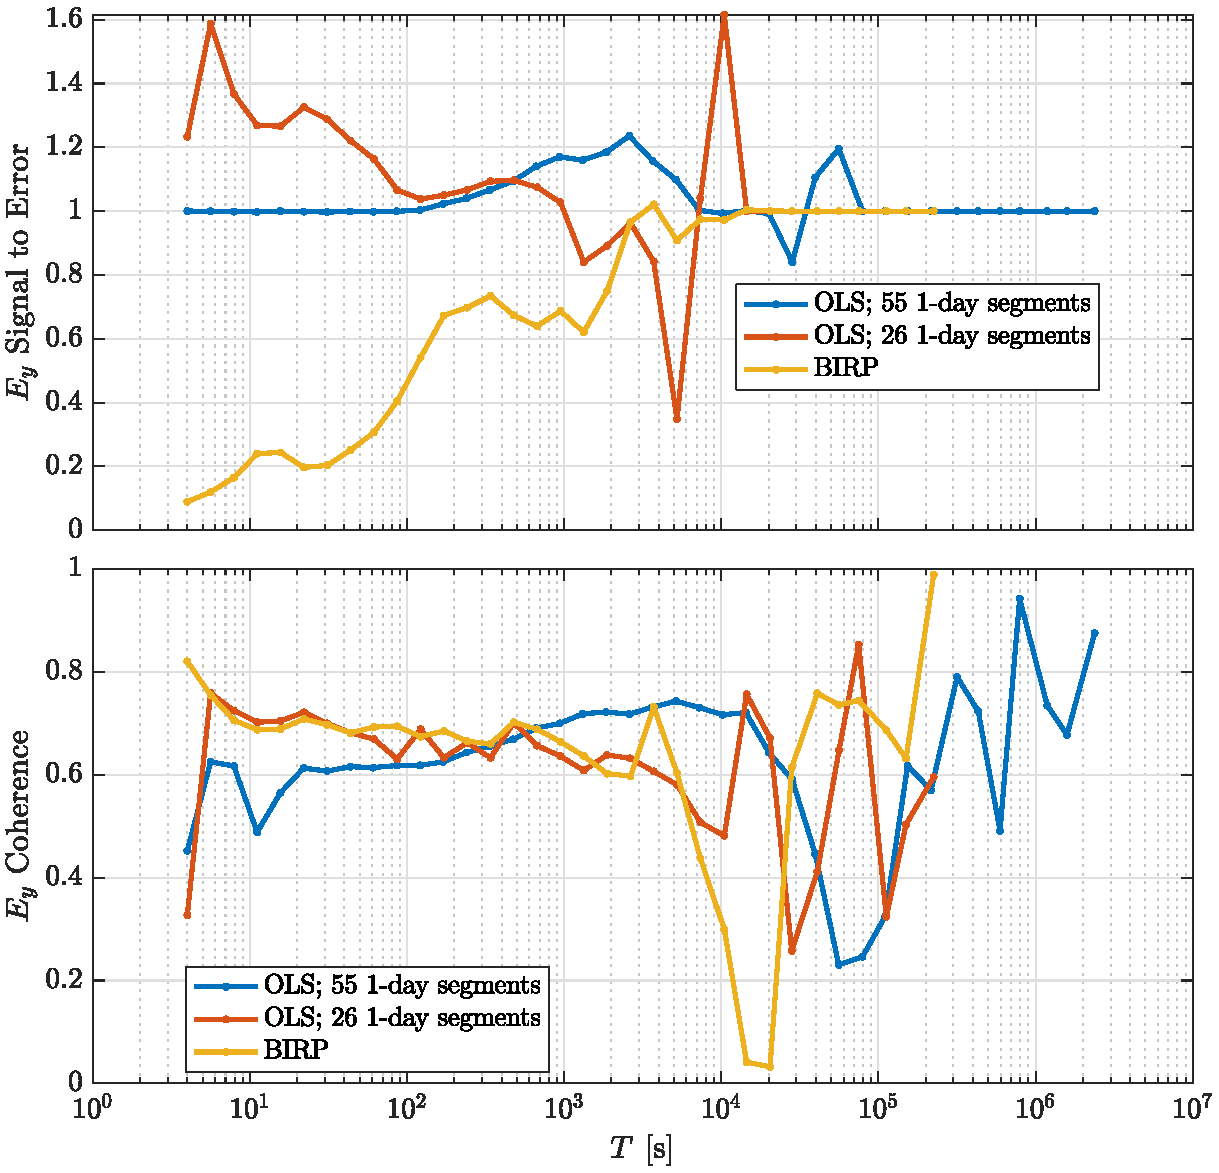
\includegraphics[width=\textwidth]{figures/KAP103_Middelpos/SN_compare-E_y.pdf}
\caption{}
\label{fig:universe}
\end{figure}

\clearpage

\begin{figure}[h!]
\centering
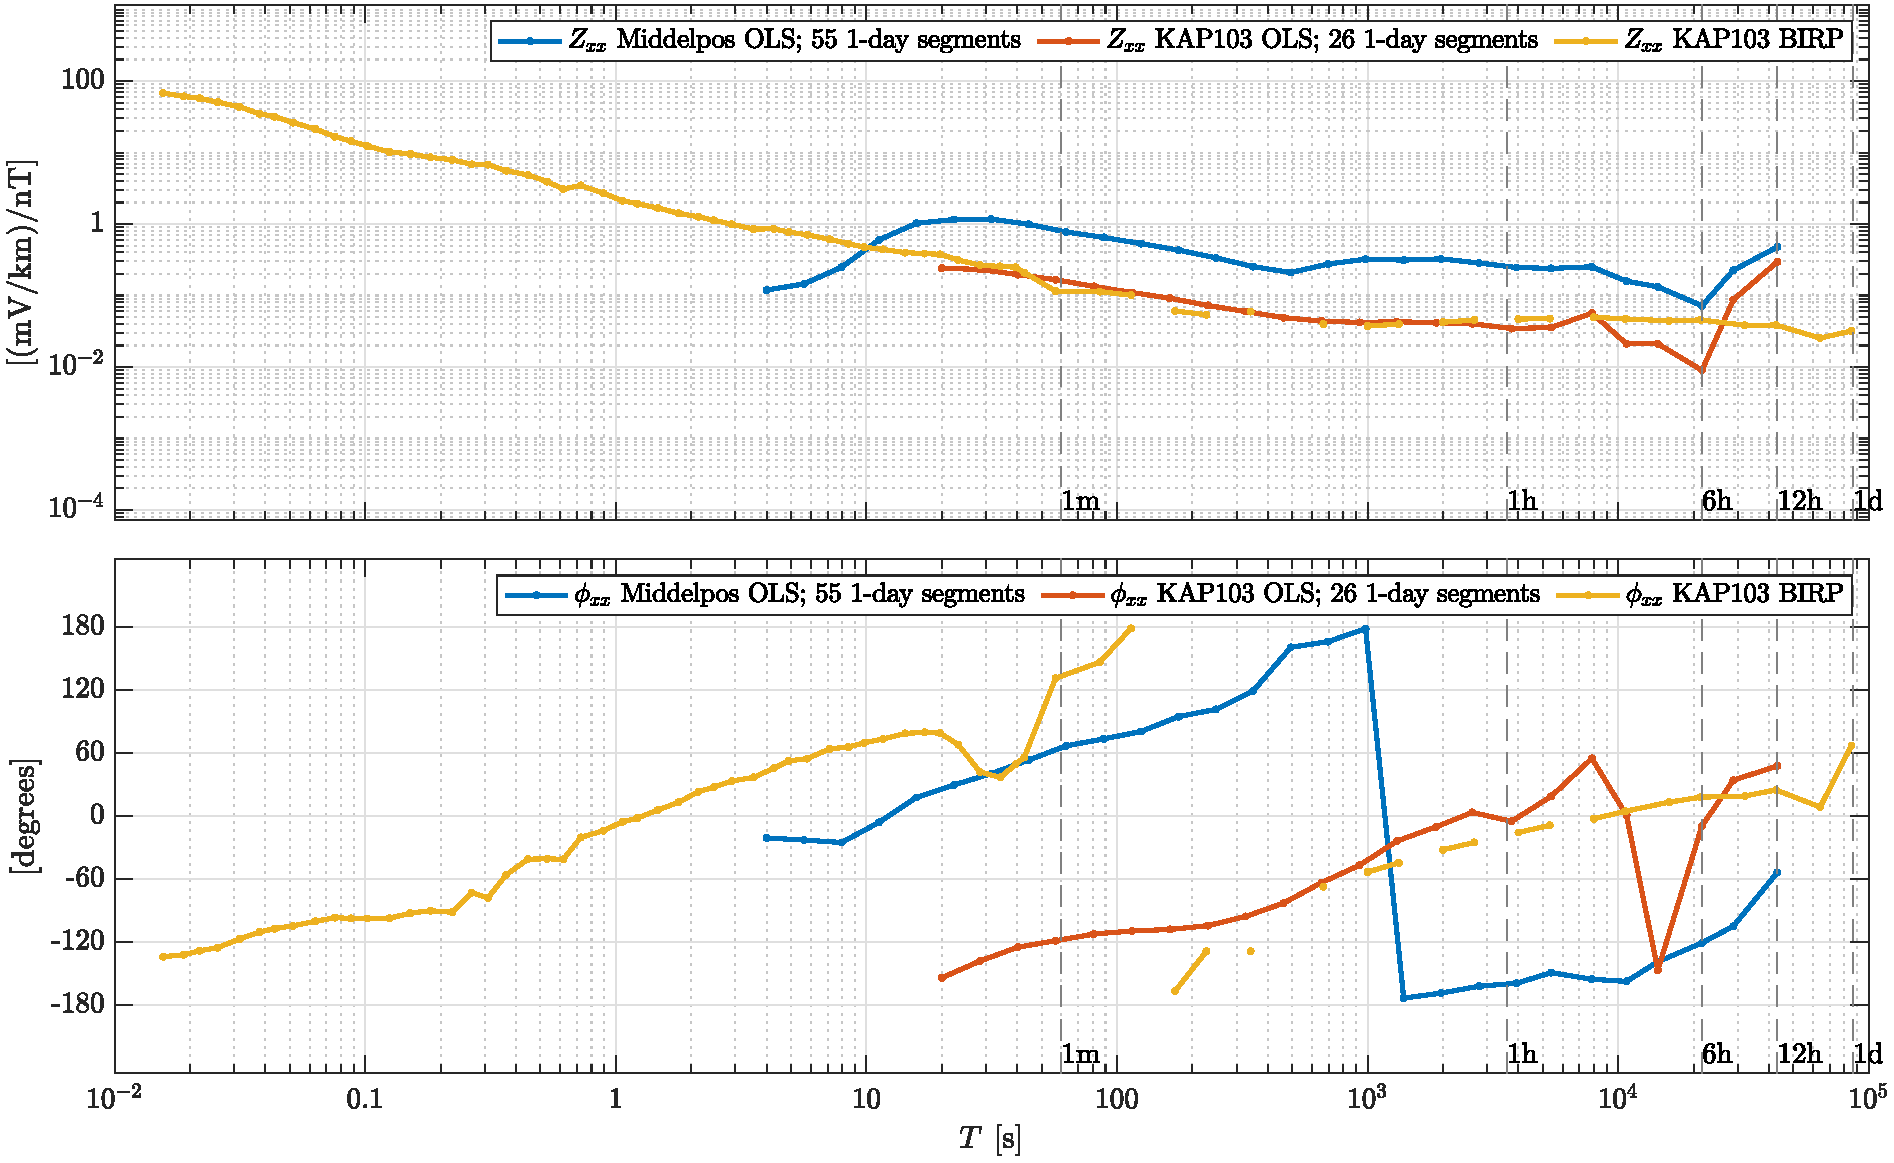
\includegraphics[width=\textwidth]{figures/KAP103_Middelpos/transferfnZ_compare-Z_xx_Magnitude_Phase.pdf}
\caption{}
\label{fig:universe}
\end{figure}

\begin{figure}[h!]
\centering
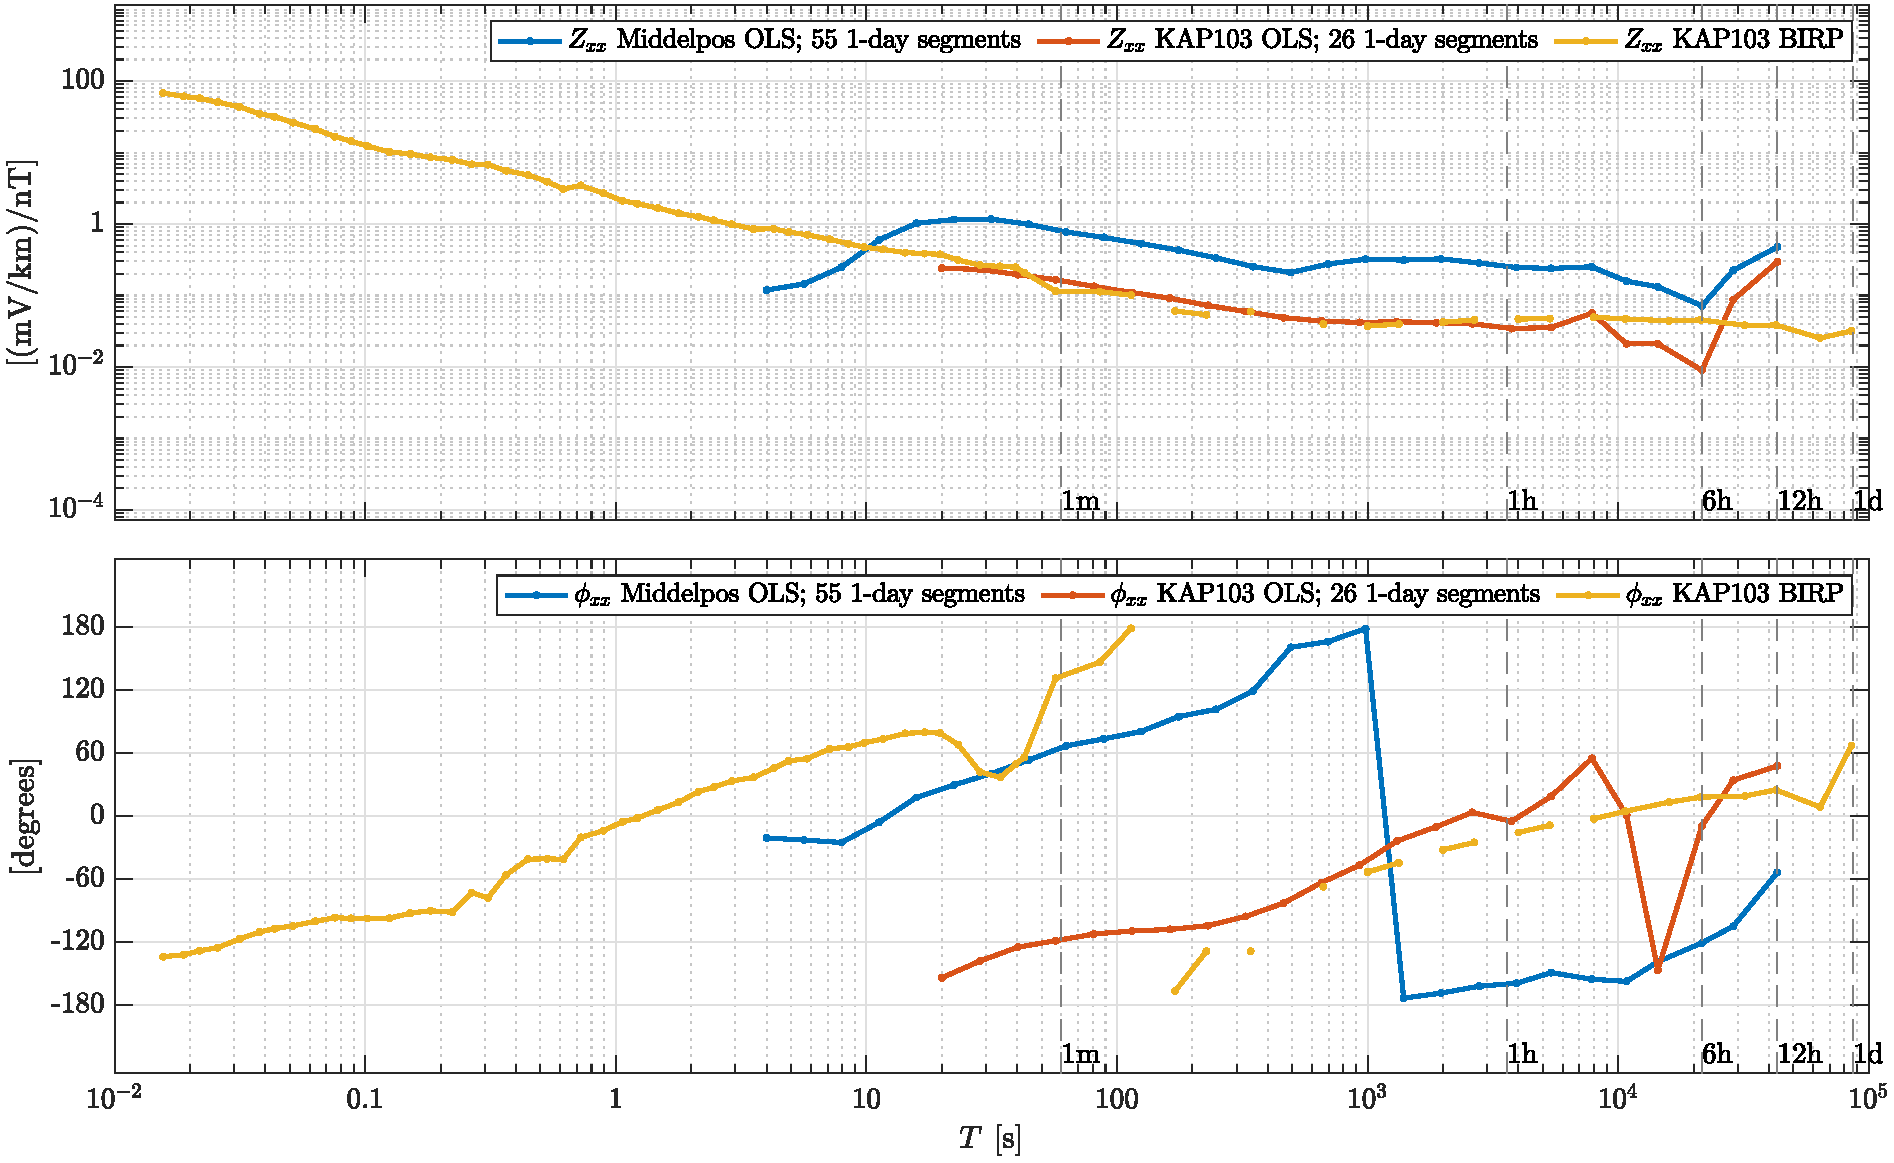
\includegraphics[width=\textwidth]{figures/KAP103_Middelpos/transferfnZ_compare-Z_xx_Magnitude_Phase.pdf}
\caption{}
\label{fig:universe}
\end{figure}

\clearpage

\begin{figure}[h!]
\centering
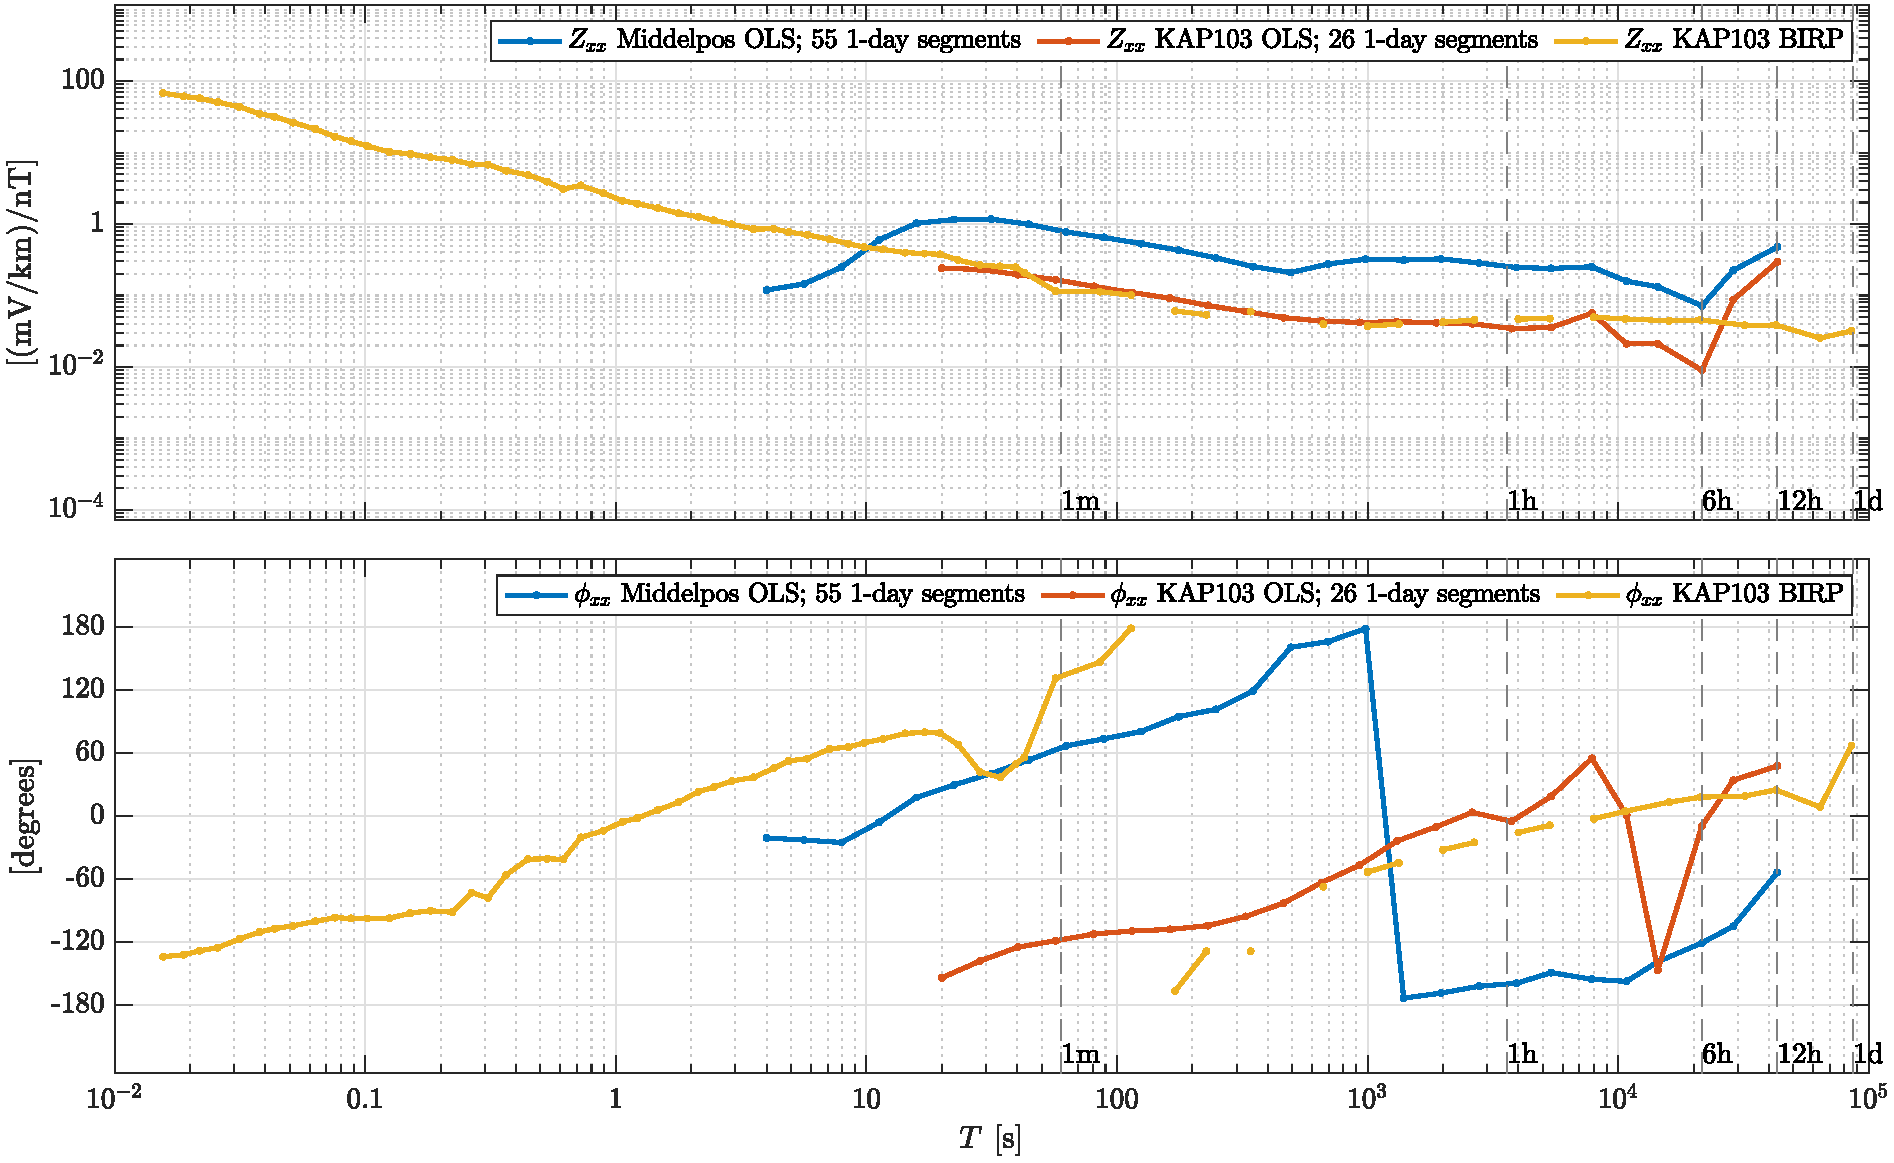
\includegraphics[width=\textwidth]{figures/KAP103_Middelpos/transferfnZ_compare-Z_xx_Magnitude_Phase.pdf}
\caption{}
\label{fig:universe}
\end{figure}

\begin{figure}[h!]
\centering
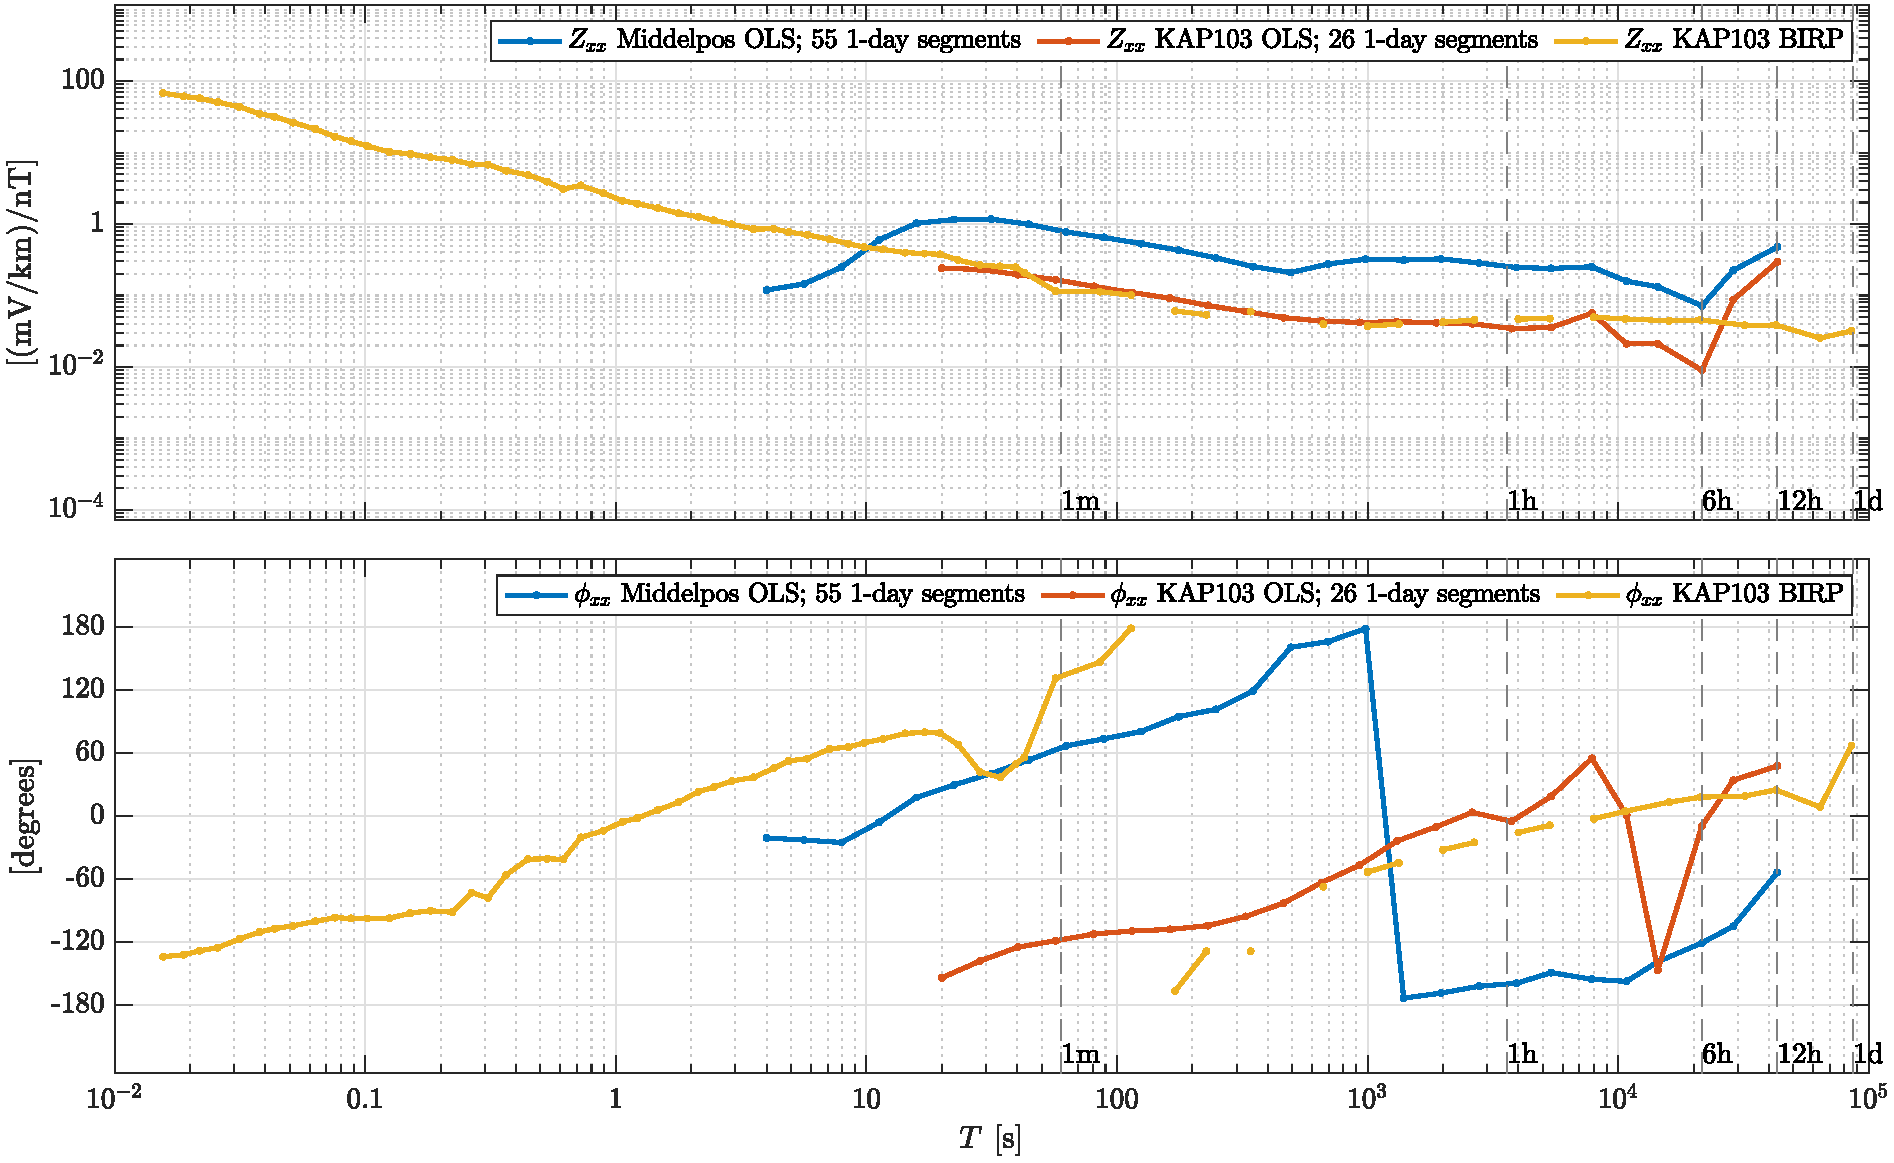
\includegraphics[width=\textwidth]{figures/KAP103_Middelpos/transferfnZ_compare-Z_xx_Magnitude_Phase.pdf}
\caption{}
\label{fig:universe}
\end{figure}

\end{document}
